\section{Experimental Results}


\subsection{Evaluation of Data Graph Formats}
In this section, we first present the space cost of three data graph formats, including CSR, hash-PCSR, and  interval-PCSR. The results are
shown in Table \ref{tab:graphsize}. We can see from Table \ref{tab:graphsize} that CSR has the smallest space among three data graph
formats. The reason is that all VIDs in CSR are contiguous and unique, while VIDs in PCSR are non-contiguous and many duplicate VIDs exist
in different edge label partitions. However, we need to transfer the whole CSR format graph to GPU in order to perform subgraph search,
which is space and time consuming. In contrast, our interval-PCSR achieves similar space cost as CSR but only needs to transfer one edge
label partition to GPU before each iteration of subgraph search. AS shown in Table \ref{tab:graphsize}, the size of the maximum edge label
partition in interval-PCSR (denoted as \emph{Max}) is greatly smaller than CSR, which makes data transfer in our approach more efficient.


\begin{table}
\centering
  \caption{Space cost of CSR, hash-PCSR, and interval-PCSR. The \emph{Max} column represents the size of maximum edge label partition in interval-PCSR. The \emph{reduce-hash} column represents the percentage of the saved space by interval-PCSR compared to hash-PCSR.}
  \label{tab:graphsize}
  \begin{tabular}{ccp{30pt}p{30pt}cp{30pt}}
  \hline
    Graph &CSR&interval-PCSR&hash-PCSR&\emph{Max}&\emph{reduce-hash}\\
    \hline
    Enron 		&1.6MB	&1.7MB	&13MB	&0.6MB	&87\% \\
    FirstMM 	&1.2MB	&1.5MB	&22MB	&0.5MB	&93\% \\
    DD 			&15MB	&11MB	&139MB	&2.1MB	&87\% \\
    Gowalla 	&8.1MB	&9.4MB	&74MB	&1.9MB	&94\% \\
    Patents 	&149MB	&184MB	&1.6GB	&26MB	&89\% \\
    Reddit 		&60MB	&71MB	&901MB	&10MB	&92\% \\
    Orkut 		&906MB	&997MB	&1.94GB	&100MB	&50\% \\
    sinaweibo	&2.2GB	&2.5GB	&10GB	&256MB	&75\% \\

    \hline
  \end{tabular}
\end{table}

Our interval-PCSR can averagely reduce the space cost of hash-PCSR by 83\%.The main reason for the large space cost of hash-PCSR is empty
entries in hash indexes. The hash-PCSR groups edges by their edge label, which makes VIDs in each group are non-contiguous. To find the
index of a given VID, hash-PCSR designs a hash function to map a given VID to a position that points to the neighbors of the VID. If
multiple VIDs are mapped to the same position, a sequential search has to be performed to find the true position of the VID, which is a
time-consuming operation in GPU. Therefore, hash-PCSR trades space for time and generates 30 empty entries for each VID to reduce
collisions. This method significantly reduces collisions and also incurs large space cost. For example, the largest edge label partition in
the data graph Enron contains 24737 VIDs. And hash-PCSR needs $32 \times 24737$ 32-bit variables to store hash indexes. While in our
interval-PCSR, we use one interval index to represent a range of contiguous VIDs and adopt Algorithm \ref{algo:genmap} to generate more
contiguous VIDs. For the above example, we need only one interval index with two numbers to index positions of 24737 VIDs. The first number
is the starting VID of this interval and the second number is the length of this interval. Thus, our interval-PCSR significantly reduces
the space cost of hash-PCSR.

To further evaluate the effectiveness of our interval-PCSR, we compare the searching time spent on finding neighbors of a given VID between
interval- and hash-PCSR. There is currently no applicable method that can measure the searching time inside a GPU thread without
interfering the normal execution flow. Therefore, we extract searching related codes from \SystemName and GSI, and construct two GPU
kernels using extracted codes respectively. We use the execution configuration of one thread block with one warp (32 threads) for both GPU
kernels, which enables us to avoid interference such as warp scheduling. To ensure the accuracy of the measurement, we search all VIDs of a
data graph in each edge label partition and record the searching time. The results are shown in Figure \ref{fig:searchtime}.
\begin{figure}
\centering
\includegraphics[width=\columnwidth]{./figure/accesstime.eps}
\caption{The searching time of interval- and hash-PCSR on all data graphs.}	
\label{fig:searchtime}
\end{figure}

We can see in Figure \ref{fig:searchtime} that our interval-PCSR achieves better performance than hash-PCSR in all data graphs and obtains
an average speedup of 2.4$\times$. In hash-PCSR, GSI first uses a hash function to calculate the index of a given VID, and then loads 32
indexes from global memory into shared memory. Finally, GSI finds the address of neighbors of the VID. Our approach needs to search the
given VID in intervals that are stored in shared memory and load the address of neighbors from global memory. Though our approach needs
more shared memory accesses than GSI, the accesses to shared memory in our interval-PCSR is aligned and the latency is negligible compared
to the global memory access. The main reason for the overhead of hash-PCSR is the calculation of hash indexes. More specifically, the
modulo operation in the hash function accounts for a large portion of execution time of the hash operation. We replace the variable divisor
of the modulo operation with a fixed constant and present the searching time in Figure \ref{fig:searchtime}. We can see that the hash-PCSR
runs much faster without the modulo operation. However, variable divisor is necessary for the modulo operation to generate correct results.

In summary, our interval-PCSR not only reduces the space cost of hash-PCSR by replacing hash indexes with interval indexes, but also
reduces the searching time by eliminating hash calculation.


\section{Evaluation}
In this section, we conduct experiments to evaluate the performance of \SystemName, GSI, and SV-match. First, we show the space cost and searching time of hash-PCSR and interval-PCSR data graph formats generated by GSI and \SystemName respectively. Then, we demonstrate the overall performance of GSI and \SystemName. Finally, we compare \SystemName to SV-match to demonstrate the effectiveness of parallel vertex matching.

\subsection{Experimental Setup}


\subsection{Comparison of \SystemName and GSI} \label{sec:comparegsi}
\begin{figure*}
\centering
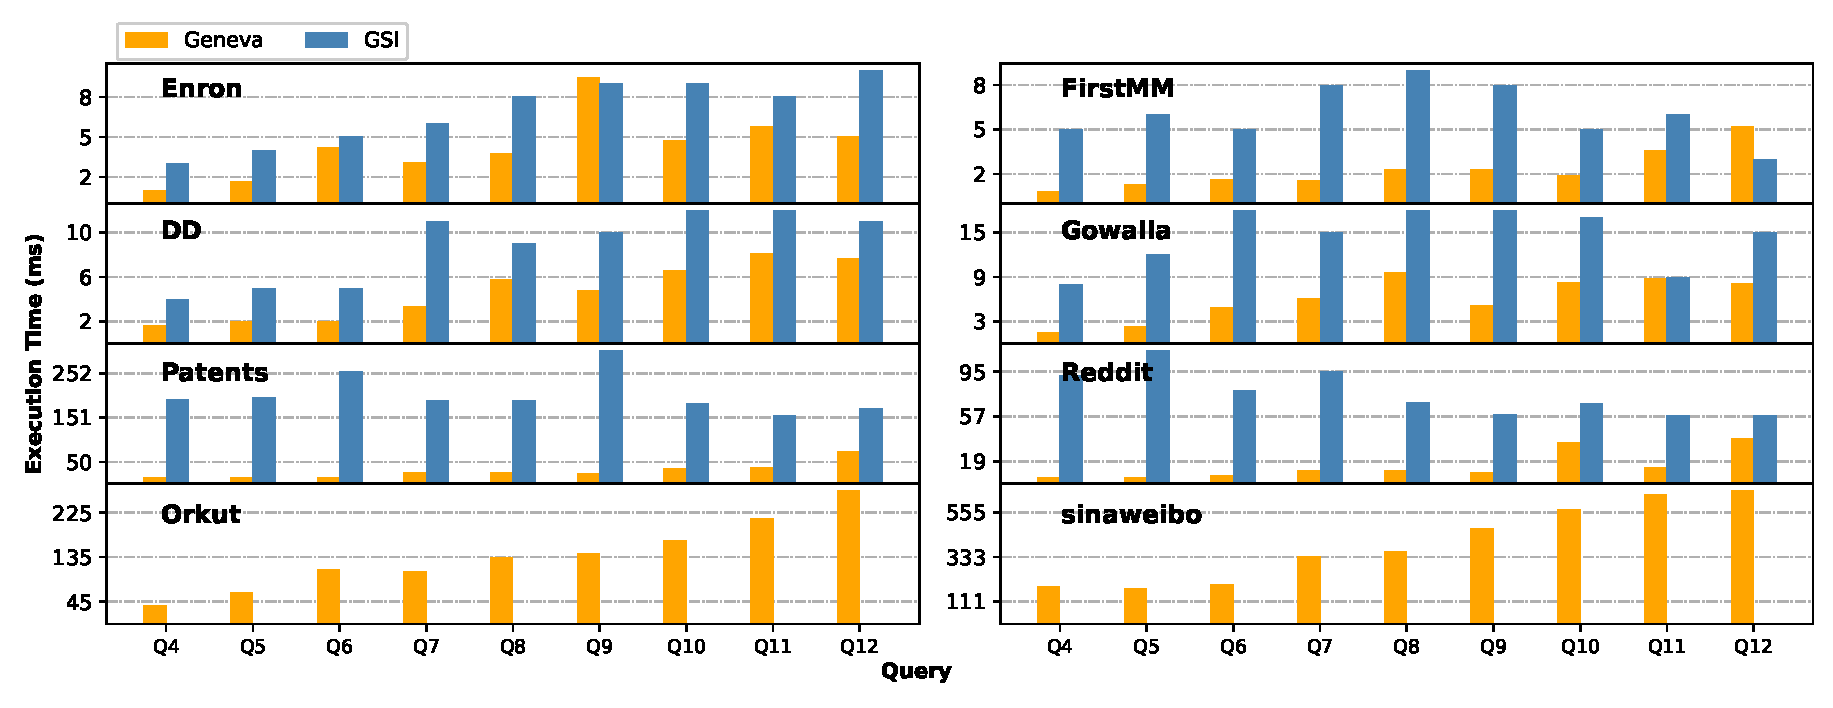
\includegraphics[width=\textwidth]{./figure/overperformance.eps}
\caption{Execution times of \SystemName and GSI for searching nine query graphs on each of eight data graphs.}	
\label{fig:overallperf}
\end{figure*}

\begin{figure}
\centering
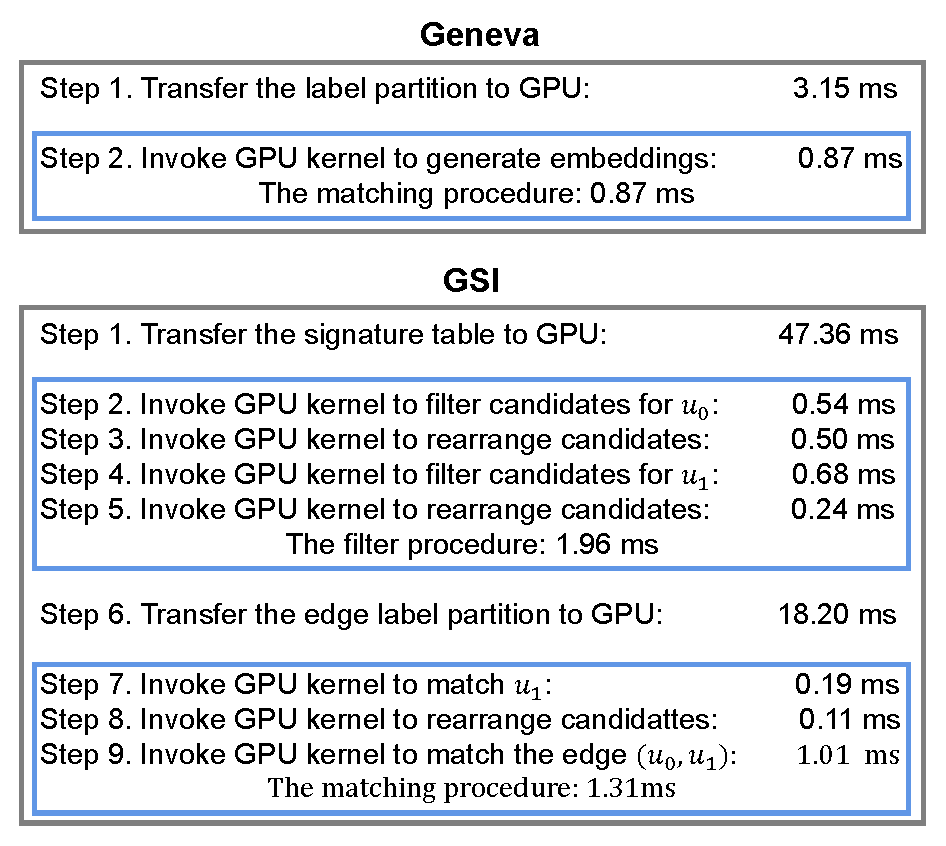
\includegraphics[width=\columnwidth]{./figure/comparegsi.eps}
\caption{The execution times of main procedures of \SystemName and GSI.}	
\label{fig:compdvgsi}
\end{figure}
In this section, we present the overall performance of \SystemName and GSI on eight data graphs. For each data graph, we first use random walk to extract nine query graphs from it with vertex count ranging from 4 to 12, and then employ both methods on the data graph to match the generated nine queries. The runtime results are shown in Fig \ref{fig:overallperf}. GSI runs out of GPU memory in data graphs Orkut and sinaweibo.

Our approach outperforms GSI in almost all test cases and achieves an average speedup of $5\times$. The maximum speedup of our approach over GSI can be up to $22.5\times$. As can be seen, GSI outperforms our approach in two test cases. The reasons can be explained as follows: (1) When matching $Q9$ in the data graph Enron, GSI finds 620K embeddings while \SystemName finds over 19M embeddings. GSI misses a vast number of embeddings, which makes it more faster than \SystemName; (2) When matching $Q12$ in the data graph FirstMM, GSI exits after matching three vertices because no embeddings can be matched, while \SystemName matches all vertices and edges of $Q12$ and finds one embedding. Therefore, \SystemName is slower than GSI in this test case.

In Figure \ref{fig:overallperf}, the average speedup of \SystemName over GSI is $7\times$ for small queries ($Q4$-$Q7$), while it is $3\times$ for large queries ($Q8$-$Q12$). The reason behind this phenomenon is explained as follows. \SystemName can generate an initial extension phase with at least two vertices. Additionally, if there exist vertices that form one of matching patterns 1-4, our approach can generate an initial extension phase with three vertices. Therefore, only two or three extension phases are needed for small queries to complete the matching process. This saves a large number of global memory accesses, which significantly accelerate the matching process for small query graphs.

To find out dominating factors for the superiority of \SystemName over GSI, we analyze detailed runtimes of each procedure of both methods. We employ \SystemName and GSI to match the query graph $Q4$ in the data graph Patents, and present the runtime of each step in Figure \ref{fig:compdvgsi}. We only show runtimes of procedures invoked when matching the first two query vertices, $u_0$ and $u_1$. The reasons are twofold: (1) In GSI, steps after matching $u_0$ and $u_1$ repeat steps 6-9 of Figure \ref{fig:compdvgsi}, and exhibit similar performance; (2) The runtimes of following steps are affected by the number of intermediate embeddings. Only when matching the first two vertices, we can make sure that both \SystemName and GSI process the same number embeddings.

We show the runtimes of \SystemName and GSI in Figure \ref{fig:compdvgsi}, and reveal three root causes of inefficiency of GSI compared to \SystemName.
\begin{itemize}
  \item GSI utilizes a filter procedure to prune candidates for each query vertex. It takes 1.96 ms to complete, which is twice the runtime of the matching procedure of \SystemName. Moreover, GSI needs to transfer the signature table to GPU before running the filter procedure. The runtime of data transfer along takes up 68\% runtime of GSI. This is because the signature table uses 64 bytes for each vertex in the data graph to store neighbor information, which results in a large data structure. Compared to GSI, \SystemName does not employ the filter procedure due to its inefficiencies in time and space.

  \item Before the matching procedure, both methods need to transfer the edge label partition to GPU. However, the execution time of data transfer in GSI is six times slower than \SystemName. The reason is explained as follows. GSI builds a hash-PCSR data structure for each edge label partition and inserts 30 empty entries into hash indexes to reduce the number of collisions. Consequently, hash-PCSR occupies a large portion of memory space, and thus takes a much longer time to be moved to GPU than the interval-PCSR of \SystemName.

  \item In the matching procedure, GSI invokes three GPU kernels to match the query vertex $u_1$, rearrange intermediate embeddings, and match the edge between $u_0$ and $u_1$, respectively. The kernel invoked in step 9 consumes most of the runtime of the matching procedure because it uses multiple time-consuming operations, such as thread block level synchronization and memory copy operations, inside the GPU kernel to maintain load balance. The four-layer load balance scheme of GSI can reduce the load imbalance greatly but also incur significant overhead. Different from GSI, our load balance scheme is simple yet effective. Only when there is no embeddings left, load imbalance can occur.
\end{itemize}

In summary, our approach obtains superior performance over GSI which is the state-of-the-art subgraph matching approach on GPU.

\subsection{Comparison of \SystemName and SV-match} \label{sec:comparesv}
\begin{figure*}
\centering
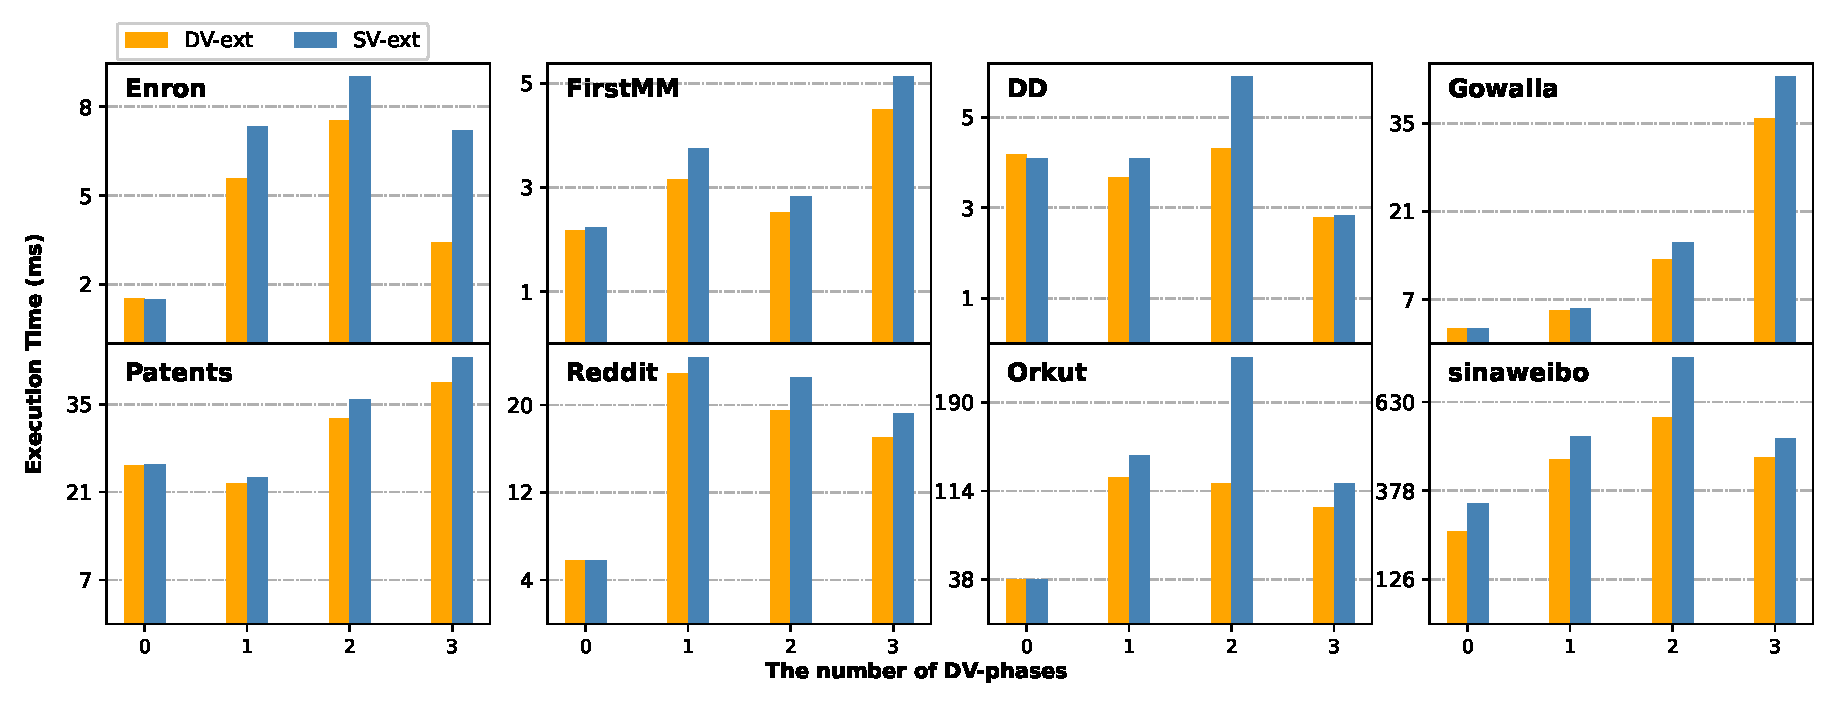
\includegraphics[width=\textwidth]{./figure/compareSV.eps}
\caption{Execution times of \SystemName and SV-match for different number of extension phases that contain matching patterns 1-7.}	
\label{fig:compareSV}
\end{figure*}
To further evaluate the performance of \SystemName, we demonstrate how the number of extension phases that contain matching patterns 1-7 affect the performance of \SystemName. For simplicity, we call the extension phase that contains one of matching patterns 1-7 the PV-phase, and the extension phase that contains the matching pattern 0 the SV-phase. For each data graph, we use random walk to extract several query graphs and classify them into different categories by the number of PV-phase, and select one query graph from each category for each data graph. The results are shown in Figure \ref{fig:compareSV}.

We can see in Figure \ref{fig:compareSV} that when the number of PV-phase is 0, both \SystemName and SV-match exhibit similar performance because all phases of both methods are the same. When the number of pV-phase is 1, 2, and 3, \SystemName improves the performance of SV-match by 11.3\%, 20.2\%, and 16.3\% respectively. In the data graph DD, the performance of \SystemName is very close to SV-match because there is only one embedding that is isomorphic to the query graph and the runtime is too short to observe the difference between \SystemName and SV-match.
